\begin{figure}
\begin{center}
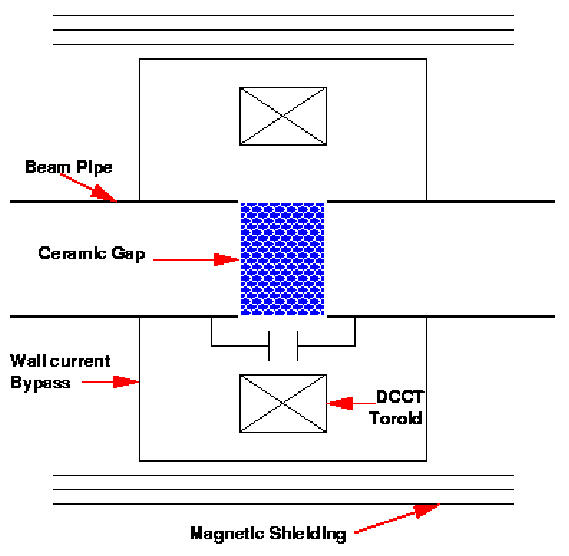
\includegraphics[width=0.75\linewidth]{./figures/dcct_schematic_cartoon}
\caption{The wall current monitor uses an insulating ceramic break in the beam pipe
similarly to the DCCT, which forces image wall currents through electronics which measure
the current frequencies. The WCM is sensitive only to bunched beams, and can measure
longitudianl profiles of bunches ~\cite{kawallfocus2005}.}
\label{fig:dcct_schematic_cartoon}
\end{center}
\end{figure}
